\documentclass[12pt]{report}
% Packages
\usepackage[utf8]{inputenc}
\usepackage{newtxtext,newtxmath}
\usepackage{geometry}
\usepackage{setspace}
\usepackage{hyperref}
\usepackage{graphicx}
\usepackage{float}
\usepackage{amsmath}
\usepackage{titlesec}
\usepackage{tikz}
\usepackage{enumitem}
\usetikzlibrary{shapes.geometric, arrows.meta, positioning}
\usepackage{algorithm}
\usepackage{algpseudocode}
\usepackage{amsmath}   % For math symbols
\usepackage{microtype} % For better typography


\usepackage{fancyhdr}
\usepackage{microtype}
\usepackage{etoolbox}

\usepackage{titlesec}

% -------------------------------
% Page Style
% -------------------------------
\pagestyle{fancy}
\fancyhf{}
\fancyfoot[C]{\thepage}
\renewcommand{\headrulewidth}{0pt}

% Margins
\geometry{
  a4paper,
  left=3.5cm,
  top=2.5cm,
  right=1.25cm,
  bottom=1.25cm,
  footskip=0cm
}


% -------------------------------
% Fix for Unnumbered Chapters (like Abstract, Acknowledgement)
% -------------------------------
\makeatletter
\renewcommand{\@makeschapterhead}[1]{%
  \vspace*{-20pt} % Adjust this to control spacing from top
  {\parindent \z@ \centering
    \normalfont\large\bfseries \hyphenpenalty=10000 \exhyphenpenalty=10000
    #1\par\nobreak\vskip 20pt
  }}
\makeatother

% -------------------------------
% Chapter Title Custom Format
% -------------------------------
\makeatletter
\renewcommand{\@makechapterhead}[1]{%
  \vspace*{-40pt} % spacing above chapter
  {\parindent \z@ \centering \normalfont
    \large\bfseries \hyphenpenalty=10000 \exhyphenpenalty=10000
    Chapter \thechapter:~#1\par\nobreak\vskip 30pt
  }}
\makeatother

% -------------------------------
% Section & Subsection Font Sizes
% -------------------------------
\titleformat{\section}
  {\normalfont\bfseries\fontsize{12}{14}\selectfont}
  {\thesection}{1em}{}

\titleformat{\subsection}
  {\normalfont\bfseries\fontsize{12}{14}\selectfont}
  {\thesubsection}{1em}{}


% -------------------------------
% Clean List Spacing
% -------------------------------
\setlist[itemize]{topsep=0pt, itemsep=3pt}
\setlist[enumerate]{topsep=4pt, itemsep=4pt}



\begin{document}

% Title Page
\begin{titlepage}
\begin{center}
    
    \textbf{\Large FINAL PROGRESS REPORT}\\[0.5cm]

    {\large ON}\\[0.5cm]

    {   \centering
        {\fontsize{18}{22}\selectfont\textbf{Automated Tuberculosis Detection and Severity Assessment using Chest X-Ray Images}\par}
        \vspace{1cm}
    }
    
    {\large SUBMITTED IN PARTIAL FULFILLMENT FOR THE AWARD OF DEGREE OF}\\[0.75cm]
    \textbf{\Large BACHELOR OF TECHNOLOGY}\\[0.2cm]
    
    {\fontsize{16}{18}\selectfont Computer Science \& Engineering}\\[1.5cm]

    \textbf{\fontsize{12}{14}\selectfont SUBMITTED BY:}\\[0.25cm]
    {\fontsize{12}{14}\selectfont CHANDAN (2203415)\\ JASPREET SINGH (2203473)\\ SRIJAN SINGH (2203565)\\[1cm]

    \textbf{\fontsize{12}{14}\selectfont UNDER THE GUIDANCE OF:}\\[0.25cm]
    Er. JASDEEP KAUR \\[1cm]


    % Insert GNDEC Logo
    \includegraphics[width=0.3\textwidth]{Images/gndec_logo.png} 
    \\[1cm]
    
    
    % \vspace{1.5cm}
    % \begin{minipage}[t]{0.45\textwidth}
    % \raggedright
    % \textbf{Submitted By:}\\[0.2cm]
    % Harsh (2203455)\\
    % Karan Kashyap (2203481)\\
    % Manish Choudhary (2203495)
    % \end{minipage}
    % \hfill
    % \begin{minipage}[t]{0.45\textwidth}
    % \raggedleft
    % \textbf{Submitted To:}\\[0.2cm]
    % Prof. Diana Nagpal\\
    % Department of Computer Science\\
    % GNDEC Ludhiana
    % \end{minipage}\\[2cm]

    
    
    
    % \textbf{\Large DEPARTMENT OF COMPUTER SCIENCE AND ENGINEERING,}\\ [0.2cm]
    \textbf{\fontsize{16}{18}\selectfont GURU NANAK DEV ENGINEERING COLLEGE,}\\
    \textbf{\fontsize{16}{18}\selectfont LUDHIANA, 141006}\\
    {\fontsize{12}{14}\selectfont March 2026}\\
\end{center}
\end{titlepage}


\pagenumbering{roman} 
\setcounter{page}{1} 

% Abstract
\chapter*{Abstract}
\doublespacing

Tuberculosis remains one of the deadliest infectious diseases in the world, killing well over a million people every year. Chest X-rays are the go-to screening tool in most countries, but reading them accurately requires trained radiologists --- professionals who are in extremely short supply across high-burden regions. In recent years, deep learning models have shown they can detect TB from X-ray images with impressive accuracy. However, nearly all of these models simply output a yes-or-no answer: the patient either has TB or does not. What they fail to provide is any indication of \textit{how bad} the disease actually is, which is something clinicians need in order to plan treatment.

This project was built to fill that gap. We developed a deep learning system that does two things at once from a single chest X-ray: it classifies whether the patient has active TB, and it estimates a severity score that quantifies how much of the lung is affected. The model uses a hybrid neural network architecture that combines convolutional and attention-based components to capture both local patterns and broader spatial context within the lung field. One of the biggest obstacles we ran into was the lack of severity-labelled training data, since very few public datasets include that kind of annotation. We addressed this through a structured approach to generating training labels from multiple annotation sources of varying quality.

The system was evaluated using cross-validation techniques with patient-level grouping to prevent data leakage, and the results met or exceeded most of our performance targets. On the deployment side, the trained model is packaged into a web-based dashboard that presents the findings in a visual, interactive format --- accessible within a few seconds on a regular laptop. The end result is a practical, interpretable diagnostic support tool that could realistically be used in TB screening programmes, especially in places where radiologist access is limited.

% Acknowledgment
\chapter*{Acknowledgment}
\doublespacing

We would like to sincerely thank Dr. Sehijpal Singh, Principal of Guru Nanak Dev Engineering College (GNDEC), Ludhiana, for giving us the platform and the academic resources to carry out this major project.

Our heartfelt thanks go to Dr. Kiran Jyoti, Head of the Computer Science and Engineering Department at GNDEC Ludhiana, who supported and encouraged us throughout the development process.

We owe a great deal to our project guide, \textbf{Er. Jasdeep Kaur}, whose guidance shaped every phase of this work. She was always available for discussions, pointed us in the right direction when we were stuck, and helped us stay on track from start to finish. This project would not have turned out the way it did without her mentorship.

We are also thankful to the other faculty members and our friends who gave us feedback and suggestions along the way. And finally, a big thank you to our families for being patient with us and for their constant support during the entire journey.

\vspace{1cm}

\textbf{Chandan} \newline
\textbf{Jaspreet Singh} \newline
\textbf{Srijan Singh}

% TOC, LOF, LOT
\tableofcontents
\listoffigures
\listoftables
\newpage
\pagenumbering{arabic}
\setcounter{page}{1}

% Chapter 1: Introduction
\chapter{Introduction}
\doublespacing

\section{Project Overview}

Tuberculosis, commonly known as TB, is caused by the bacterium \textit{Mycobacterium tuberculosis} and spreads through the air. The World Health Organization (WHO) reports that TB is still the second deadliest infectious disease on the planet --- around 10.6 million people got sick with it in 2022, and roughly 1.3 million died. The burden falls hardest on low- and middle-income nations, where there simply are not enough trained radiologists to read the volume of chest X-rays being produced.

Chest X-rays (CXRs) are by far the most widely used tool for TB screening. But interpreting them well takes years of clinical training, and in countries where TB is most common, that expertise is scarce. This is where deep learning comes in --- automated analysis of CXRs could help close the diagnostic gap. The trouble is, most existing AI systems for TB treat it as a straightforward binary problem: they look at an X-ray and say either ``yes, TB'' or ``no, not TB.'' That is useful for first-pass screening, but it tells the clinician nothing about \textit{how severe} the disease is.

In practice, especially under WHO treatment guidelines, doctors rely on the \textbf{Timika score} to gauge disease burden. This is a validated metric that ranges from 0 to 140 and is calculated based on how much of the lung area shows visible lesions and whether cavitation is present. If a system could predict this score straight from a chest X-ray, it would give clinicians far more actionable information than a simple positive/negative label.

That is exactly what this project sets out to do. We built a \textit{Multi-Task} deep learning system that handles TB classification and Timika severity regression simultaneously, all from a single CXR image. At its core is a hybrid architecture: an Inception-v3 convolutional backbone extracts fine-grained local features like lesion texture and nodule margins, while a Transformer encoder sitting on top captures broader spatial patterns such as how disease is distributed across both lungs. We also had to deal with the reality that severity annotations are hard to come by, so we built a multi-tier pipeline to generate training labels from whatever annotation sources were available. The final trained model is deployed through a FastAPI web dashboard where users can upload an X-ray and get back a TB probability, a severity score, and a Grad-CAM heatmap --- all in real time.

\section{Project Category}

This project sits at the intersection of \textbf{Artificial Intelligence and Medical Imaging}. More specifically, it touches on several sub-domains:

\begin{itemize}
    \item \textbf{Multi-Task Learning (MTL):} Instead of building two separate models, we train a single network with two output heads --- one for TB classification and one for severity regression. The shared feature layers learn representations that benefit both tasks at the same time.

    \item \textbf{Hybrid Deep Architectures:} We combine a CNN (for picking up local spatial patterns in the image) with a Transformer encoder (for reasoning about the image as a whole). Neither component alone would be as effective as both working together.

    \item \textbf{Weakly Supervised and Semi-Supervised Learning:} Since most of our training data does not come with pixel-level severity annotations, we use a mix of polygon annotations, bounding box labels, and Grad-CAM++ pseudo-labels to construct severity scores from whatever annotation format is available.

    \item \textbf{Explainable AI (XAI) in Healthcare:} We generate Grad-CAM heatmaps at inference time so that clinicians can actually see which parts of the lung the model is paying attention to. This kind of transparency is essential in any medical application.
\end{itemize}

From the engineering side, this project covers the full pipeline end to end: collecting and merging datasets, processing annotations, training the model on Kaggle's T4 $\times$2 GPUs, evaluating with out-of-fold predictions, and deploying locally through a FastAPI backend with a plain HTML/JS frontend.

\section{Problem Formulation}

Most deep learning models for TB right now are binary classifiers --- they look at a chest X-ray and decide whether TB is present or not. While that is a useful first step for screening, it throws away a lot of the information that is actually visible in the image. In particular, the following questions go completely unanswered by a simple positive/negative output:

\begin{itemize}
    \item How much of the lung tissue is actually affected by disease?
    \item Is there cavitation, which might point to advanced or drug-resistant TB?
    \item If we compare two X-rays taken months apart, is the patient getting better or worse?
\end{itemize}

The \textbf{Timika score} was designed to answer exactly these kinds of questions. But to train a model that predicts it, you need dense, pixel-level annotations showing where lesions are --- and that kind of data is expensive to create and almost never available at large scale. Most publicly available TB datasets give you nothing more than a binary label per image. The Shenzhen dataset is a rare exception, offering polygon-level lesion annotations, but it only covers a few hundred cases. Trying to train a severity regression model on that alone is not realistic.

So the core question driving this project is: \textit{How do you build a reliable TB severity regressor when you only have dense lesion annotations for a small fraction of your training data?}

The main technical hurdles we faced along the way include:
\begin{enumerate}
    \item \textbf{Label Scarcity:} Proper Timika scores are only available for about 336 Shenzhen cases. Thousands of other TB-positive images have no severity information at all.
    \item \textbf{Annotation Heterogeneity:} The annotations we had access to came in very different formats --- pixel-level polygons from Shenzhen, bounding boxes from TBX11K, and just binary labels from Montgomery. These cannot be directly mixed without some processing.
    \item \textbf{Multi-Task Balancing:} When you train classification and regression together, one task can easily overpower the other in the loss function, causing the weaker task to stall.
    \item \textbf{Model Generalization:} The model needs to work across X-rays from different scanners, resolutions, and patient populations --- not just the ones it was trained on.
    \item \textbf{Clinical Interpretability:} In a medical setting, a model that just spits out a number is not enough. There has to be some visual evidence backing up the prediction, or clinicians will not trust it.
\end{enumerate}

\section{Identification of Need}

There are several real-world factors that make a tool like this genuinely needed:

\begin{itemize}
    \item \textbf{Not Enough Radiologists:} The WHO estimates a global shortfall of over 4 million health workers, and radiologists are among the hardest to find in TB-heavy regions. An AI system that pre-screens X-rays could let a single radiologist handle a much larger caseload.

    \item \textbf{Current AI Tools Fall Short:} Tools like CAD4TB and qXR are already being used in some clinical settings, but they only give a probability of TB being present. They do not produce a severity metric like the Timika score, which limits how useful they are for treatment planning.

    \item \textbf{Treatment Takes Months:} Standard TB treatment runs at least 6 months. During that time, doctors want to track whether the patient is improving radiologically. Right now that means having an expert read every follow-up X-ray --- something automated severity scoring could help with.

    \item \textbf{Drug-Resistant TB:} Patients with drug-resistant strains tend to show more severe disease on their X-rays. If a model can flag high-severity cases automatically, it could help prioritise which patients need further drug-resistance testing.

    \item \textbf{Large-Scale Research:} Being able to score severity automatically would open the door to retrospective studies across entire TB cohorts --- work that currently requires years of manual annotation by experts.
\end{itemize}

\section{Existing Systems}

A number of existing systems tackle parts of the TB screening problem. Understanding what they do well --- and where they fall short --- helped shape the design of our system.

\subsection*{1. CAD4TB (Delft Imaging)}
CAD4TB is a commercial tool that analyses a chest X-ray and assigns it a TB probability score. It has been tested in over 20 clinical studies across Africa and Asia, and it works well as a triage tool.

\textbf{Where it falls short:}
\begin{itemize}
    \item It gives a probability score, not a severity measure. A clinician cannot tell from the output how bad the disease is.
    \item There are no heatmaps or lesion localisation --- the output is just a single number.
    \item The software is closed-source, so institutions cannot fine-tune it on their own patient data.
\end{itemize}

\subsection*{2. qXR (Qure.ai)}
qXR is a broader AI platform that reads chest X-rays for multiple findings, including consolidation, nodules, and pleural effusion.

\textbf{Where it falls short:}
\begin{itemize}
    \item It classifies individual findings but does not produce an overall severity score like Timika.
    \item It requires a commercial license, which puts it out of reach for many low-resource settings.
\end{itemize}

\subsection*{3. DenseNet-121 Baseline (Wang et al., CheXNet)}
CheXNet~\cite{ref6} showed that a 121-layer DenseNet could match or beat radiologists on pneumonia detection. Later work adapted similar architectures for TB.

\textbf{Where it falls short:}
\begin{itemize}
    \item It is a single-task binary classifier --- no severity estimation.
    \item The Global Average Pooling layer throws away all spatial information, which is exactly what you need for computing severity.
    \item No regression capability whatsoever.
\end{itemize}

\subsection*{What is Missing Overall}
\begin{itemize}
    \item There is no open-source system that does both TB classification and Timika severity regression at the same time.
    \item Nobody has systematically used a polygon $\rightarrow$ bounding box $\rightarrow$ Grad-CAM pseudo-label pipeline for this particular problem.
    \item Hybrid CNN-Transformer architectures have not been tried for this clinical task before.
\end{itemize}

\section{Objectives}

We set out with the following concrete goals for this project:
\begin{enumerate}
    \item Bring together three publicly available CXR datasets (Shenzhen, Montgomery, and TBX11K) into one unified training set, with consistent metadata and patient IDs that do not clash across datasets.

    \item Build a severity label generation pipeline that can produce Timika scores for TB-positive images regardless of what kind of annotation they originally came with.

    \item Design and implement a hybrid CNN-Transformer model with an Inception-v3 backbone, Efficient Channel Attention, a projection bridge, and a 4-layer Transformer encoder --- all trained jointly for classification and regression.

    \item Use a Kendall--Gal--Cipolla uncertainty-weighted loss function so that the classification and regression objectives balance themselves automatically during training, without us having to manually tune loss weights.

    \item Hit our target performance numbers: AUROC of at least 0.92 for classification, and MAE of 15 or less for Timika severity regression on held-out validation folds.

    \item Package the trained model into a web dashboard that shows TB probability, the severity score, and a Grad-CAM heatmap --- all within 3 seconds of uploading an image.
\end{enumerate}

\section{Proposed System}

At a high level, the system we built is a complete end-to-end pipeline made up of five main components. Each one is described in detail later in Chapters~3 and~4:

\begin{enumerate}
    \item \textbf{Preprocessing Module} --- Takes raw CXR images and runs them through lung segmentation, cropping, and contrast enhancement to produce clean, standardised inputs (Section~4.1).
    \item \textbf{Severity Labelling Engine} --- Computes Timika severity scores for all TB-positive images by pulling from whichever annotation source is available for that image (Section~4.2).
    \item \textbf{Hybrid CNN-Transformer Model} --- The neural network itself, which jointly predicts TB status and severity from a single preprocessed image (Section~4.3).
    \item \textbf{Training Curriculum} --- A staged training strategy that progressively unfreezes the model and uses automatic loss balancing (Section~4.5).
    \item \textbf{Inference Dashboard} --- A web interface where clinicians can upload X-rays and see predictions with visual explanations in real time (Section~4.7).
\end{enumerate}

\section{Scope of the Project}

We wanted to be clear about what this project does and does not cover.

\subsection{In Scope}
\begin{itemize}
    \item Classifying chest X-rays as either active TB or normal --- covering both posterior-anterior (PA) and anterior-posterior (AP) views.
    \item Predicting a quantitative severity score using the Timika system (scale of 0 to 140).
    \item A preprocessing pipeline that automatically segments the lungs, crops to the lung region, and normalises contrast.
    \item Generating severity labels from three different types of annotations: polygon masks, bounding boxes, and Grad-CAM++ pseudo-labels.
    \item Training exclusively on publicly available datasets (Shenzhen, Montgomery, TBX11K).
    \item Deploying the model as a local web application that runs in any standard browser.
    \item Producing Grad-CAM visual explanations overlaid on the input X-ray.
\end{itemize}

\subsection{Out of Scope}
\begin{itemize}
    \item Diagnosis of non-TB pulmonary conditions (e.g., pneumonia, lung cancer, COVID-19).
    \item Processing of lateral-view or CT scan images.
    \item Paediatric TB detection, which presents distinct radiological patterns.
    \item Integration with hospital PACS (Picture Archiving and Communication Systems) or HL7/FHIR electronic health record standards.
    \item Regulatory approval or clinical trial validation.
    \item Multi-language support in the web interface.
\end{itemize}

\section{Organization of the Report}

The rest of this report is laid out as follows:

\begin{itemize}
    \item \textbf{Chapter 2 --- Requirement Analysis and System Specification:} Covers the feasibility study, software requirement specification, and the development lifecycle model we followed.
    \item \textbf{Chapter 3 --- System Design:} Describes the datasets, overall system architecture, data flow diagrams, and module breakdown.
    \item \textbf{Chapter 4 --- Methodology:} Goes into the technical details --- preprocessing, severity label generation, model architecture, loss function, training strategy, and inference pipeline.
    \item \textbf{Chapter 5 --- Results and Discussions:} Presents the evaluation framework, classification and regression results, comparative analysis, test cases, and a discussion of limitations.
    \item \textbf{Chapter 6 --- Conclusion and Future Scope:} Wraps up our contributions and outlines where this work could go next.
\end{itemize}

\section{Literature Review}

Before diving into our own approach, it is worth surveying the relevant literature and existing tools that informed our design decisions.

\subsection{Deep Learning for Medical Image Analysis}
Since the breakthrough results of Krizhevsky et al. (2012) on ImageNet, CNNs have become the dominant approach for medical image classification. For chest X-ray analysis in particular, architectures like DenseNet-121~\cite{ref6}, ResNet-50, and EfficientNet~\cite{ref7} have been shown to perform at or near radiologist level on tasks such as pneumonia detection, cardiomegaly assessment, and pleural effusion identification. A big part of why these models work so well is transfer learning: by starting from weights pre-trained on ImageNet (roughly 1.2 million natural images), the model already knows how to detect edges, textures, and shapes. These low-level features transfer surprisingly well to medical images even though the domain is quite different.

More recently, Vision Transformers (ViT)~\cite{ref8} have emerged as a serious alternative. They apply self-attention directly to image patches, which allows them to capture long-range spatial dependencies that CNNs can miss. The catch is that ViTs are data-hungry --- they lack the built-in biases (locality, translation equivariance) that make CNNs sample-efficient, so they typically need much more training data. Hybrid architectures that pair a CNN backbone with a Transformer encoder offer a middle ground: the CNN handles local feature extraction efficiently, while the Transformer adds global reasoning on top.

\subsection{TB Detection with Deep Learning}
There has been quite a bit of work on automated TB detection from CXRs. Lakhani and Sundaram (2017) showed that fine-tuned AlexNet and GoogLeNet models could achieve AUROC values above 0.95 on the Shenzhen and Montgomery datasets. Those numbers were impressive, but the datasets are small and fairly homogeneous, so it was unclear how well the models would generalise to more diverse patient populations.

The TBX11K dataset~\cite{ref1} was a step forward in that regard --- it introduced 11,200 CXR images with bounding box annotations for TB lesions, making it the largest publicly available TB dataset to date. Liu et al. (2020) used it to train object detection models (Faster R-CNN, RetinaNet) that could localise TB lesions, but they did not attempt severity quantification. The dataset's bounding boxes are helpful for localisation, but they are rough approximations of actual lesion boundaries.

On the commercial side, tools like CAD4TB (Delft Imaging) and qXR (Qure.ai) have been deployed in real clinical settings across Africa and Asia. CAD4TB has been through over 20 prospective validation studies and consistently hits sensitivity above 90\% at the WHO-recommended specificity thresholds. But these tools still only output a probability score --- they do not tell you how severe the disease is.

\subsection{Severity Quantification and the Timika Score}
The Timika score~\cite{ref2} was originally developed as a way to quantify radiological TB severity. It measures the percentage of lung area affected by visible lesions and adds a 40-point bonus if cavitation is present, giving a score between 0 and 140. Clinically, it has been validated as a predictor of treatment outcomes, the time it takes for sputum conversion, and even mortality risk.

Despite being clearly useful, very few research groups have tried to predict the Timika score automatically. The main blocker is the data: you need pixel-level lesion annotations to compute ALP (affected lung percentage), and those annotations are rarely available in public datasets. Most TB datasets only provide image-level binary labels, which makes direct supervised regression impossible without some creative workarounds.

\subsection{Weakly Supervised Learning and Pseudo-Labeling}
When you do not have fine-grained annotations, weakly supervised learning can help bridge the gap. Techniques like Class Activation Mapping (CAM) and its variants --- Grad-CAM, Grad-CAM++ --- generate spatial heatmaps from classification models, highlighting the regions that matter most for the predicted class. These heatmaps have been used as pseudo-labels for segmentation tasks in medical imaging, particularly in situations where getting a radiologist to annotate every pixel is impractical.

In our project, we use Grad-CAM++ pseudo-labels for exactly this purpose: for TB-positive images that have no spatial annotations at all, we use the heatmaps from a teacher model as approximate lesion maps to compute rough Timika scores.

\subsection{Multi-Task Learning}
Multi-task learning (MTL) is the idea of training one model on multiple related objectives at the same time. The intuition is that the shared feature layers learn more robust representations when they have to serve more than one purpose. Kendall, Gal, and Cipolla~\cite{ref3} proposed a particularly elegant approach: instead of manually setting weights for each loss term, they let the model learn task-specific uncertainty parameters that automatically balance the losses during training. Their method was originally demonstrated on scene understanding tasks (depth estimation plus semantic segmentation), and we adopted it here to balance our classification and regression losses.

% Chapter 2: Requirement Analysis
\chapter{Requirement Analysis and System Specification}
\doublespacing

\section{Feasibility Study}

Before we started building anything, we did a feasibility study to make sure the project was actually doable within the constraints of an academic setting.

\subsection{Technical Feasibility}
From a technical standpoint, there were good reasons to believe this was achievable:

\begin{itemize}
    \item \textbf{Mature Frameworks:} PyTorch is a well-established deep learning framework with solid documentation, a large community, and good GPU support (CUDA, bfloat16 mixed precision). We were not going to be fighting the tools.

    \item \textbf{Pre-trained Weights Available:} The \texttt{timm} library provides Inception-v3 weights pre-trained on ImageNet, which gave us a strong starting point for transfer learning.

    \item \textbf{Public Datasets:} Shenzhen, Montgomery, and TBX11K are all freely available through academic repositories and Kaggle. We did not need any special data agreements.

    \item \textbf{Off-the-shelf Segmentation:} The \texttt{segmentation-models-pytorch} library has a ready-made ResNet-34 U-Net for lung segmentation, saving us from having to implement that piece ourselves.

    \item \textbf{Standard Annotation Formats:} The Shenzhen polygon annotations use VIA JSON format, and TBX11K uses COCO bounding box format. Both are well-documented and easy to parse with standard Python.

    \item \textbf{Sufficient Compute:} Kaggle's free-tier T4 $\times$2 GPU environment gives us about 32 GB of GPU memory total, which was enough to train our roughly 25M parameter model with batch size 32 at 512$\times$512 resolution.
\end{itemize}

\subsection{Economic Feasibility}
One of the nice things about this project is that it cost us literally nothing:

\begin{itemize}
    \item \textbf{Software:} Every library we used --- PyTorch, timm, segmentation-models-pytorch, Albumentations, FastAPI, OpenCV --- is open-source and free.
    \item \textbf{Compute:} All training was done on Kaggle's free GPU tier (T4 $\times$2, with a 30-hour weekly quota). Inference runs on a local CPU, so there are no cloud hosting costs.
    \item \textbf{Data:} All datasets are freely available for academic research.
    \item \textbf{Deployment:} The FastAPI server runs locally on our own machines, so there is no hosting expense.
\end{itemize}

The total direct cost of the project is zero, which made it straightforward to justify from an economic standpoint.

\subsection{Operational Feasibility}
The web dashboard is deliberately simple to use. A clinician just uploads a JPEG or PNG chest X-ray and gets results back within seconds. No machine learning knowledge is needed. On the hardware side, the backend runs comfortably on any modern computer with at least 8 GB of RAM, and the frontend works in any standard web browser.

\section{Hardware and Software Requirements}

\subsection{Hardware Requirements}

\begin{table}[H]
\centering
\caption{Hardware Requirements}
\renewcommand{\arraystretch}{1.2}
\begin{tabular}{|l|l|p{6cm}|}
\hline
\textbf{Component} & \textbf{Phase} & \textbf{Specification} \\
\hline
GPU & Training & NVIDIA T4 $\times$2 (16 GB VRAM each), provided by Kaggle \\
CPU & Inference & Any modern x86-64 processor (Intel i5 / AMD Ryzen 5 or equivalent) \\
RAM & Training & 32 GB (Kaggle environment) \\
RAM & Inference & 8 GB minimum \\
Storage & Training & 50 GB (datasets + checkpoints + intermediate outputs) \\
Storage & Inference & 2 GB (model checkpoint + U-Net weights + application code) \\
Network & Training & Internet connection for Kaggle notebook execution \\
Network & Inference & Not required (fully offline local deployment) \\
\hline
\end{tabular}
\end{table}

\subsection{Software Requirements}

\begin{table}[H]
\centering
\caption{Software Dependencies}
\renewcommand{\arraystretch}{1.2}
\begin{tabular}{|l|l|p{5cm}|}
\hline
\textbf{Software} & \textbf{Version} & \textbf{Purpose} \\
\hline
Python & 3.10+ & Core programming language \\
PyTorch & 2.0+ & Deep learning framework \\
timm & 0.9+ & Pretrained model library (Inception-v3) \\
segmentation-models-pytorch & 0.3+ & U-Net lung segmentation \\
Albumentations & 1.3+ & Image augmentation pipeline \\
OpenCV & 4.8+ & Image processing and visualization \\
FastAPI & 0.100+ & REST API backend server \\
Uvicorn & 0.22+ & ASGI server for FastAPI \\
NumPy, Pandas & Latest & Data manipulation and analysis \\
Scikit-learn & 1.3+ & Metrics computation, cross-validation \\
SciPy & 1.11+ & Statistical analysis (Pearson, Spearman) \\
Matplotlib, Seaborn & Latest & Result visualization and plotting \\
HTML5 / CSS3 / JavaScript & --- & Frontend web interface \\
\hline
\end{tabular}
\end{table}

\section{Use Case Description}

The system supports two primary use cases:

\subsection{Use Case 1: Clinical Screening}
\begin{itemize}
    \item \textbf{Actor:} Clinician / Radiologist / Community Health Worker
    \item \textbf{Precondition:} The FastAPI server is running on the local machine.
    \item \textbf{Trigger:} The actor opens the web dashboard in a browser and uploads a CXR image.
    \item \textbf{Main Flow:}
    \begin{enumerate}
        \item The system validates the uploaded file (format, size).
        \item The system preprocesses the image (normalize, segment lungs, crop, CLAHE).
        \item The system runs the trained model to produce TB probability and severity score.
        \item The system generates a Grad-CAM heatmap overlay.
        \item Results are displayed: probability bar, severity badge, score, and heatmap.
    \end{enumerate}
    \item \textbf{Postcondition:} The clinician has received a quantitative assessment to inform their clinical decision.
    \item \textbf{Alternative Flow:} If lung segmentation fails, the system falls back to centre-crop preprocessing and displays a warning.
\end{itemize}

\subsection{Use Case 2: Model Retraining}
\begin{itemize}
    \item \textbf{Actor:} Machine Learning Engineer / Researcher
    \item \textbf{Precondition:} Access to a Kaggle account with GPU quota, and the project repository.
    \item \textbf{Trigger:} The actor wishes to retrain the model with updated data or hyperparameters.
    \item \textbf{Main Flow:}
    \begin{enumerate}
        \item Modify hyperparameters in the \texttt{Config} dataclass.
        \item Run \texttt{assemble.py} to regenerate the Kaggle notebook from modular cell files.
        \item Upload the notebook to Kaggle and execute with GPU acceleration.
        \item Download the resulting checkpoints and OOF evaluation metrics.
        \item Replace the checkpoint in the local deployment directory.
    \end{enumerate}
    \item \textbf{Postcondition:} The dashboard serves predictions from the updated model.
\end{itemize}

\section{Software Requirement Specification (SRS)}

\subsection{Data Requirements}
\begin{itemize}
    \item The system accepts chest X-ray images in JPEG or PNG format.
    \item Input image resolution must be at least 128$\times$128 pixels.
    \item Training data is sourced from four curated public datasets totalling approximately 19,000 images.
    \item All training images are standardized to 512$\times$512 pixels after lung cropping.
\end{itemize}

\subsection{Functional Requirements}
\begin{itemize}
    \item The system shall accept a CXR image upload via a web interface.
    \item The system shall segment the lung field and crop the image to the lung region automatically.
    \item The system shall output a TB classification probability between 0 and 1.
    \item The system shall output a Timika severity regression score between 0 and 140 for TB-positive predictions.
    \item The system shall generate and display a Grad-CAM heatmap overlaid on the original CXR image.
    \item The system shall display a severity badge (Normal / Mild / Moderate / Severe) based on the predicted score.
    \item The severity score shall be forced to zero for images classified as TB-negative.
\end{itemize}

\subsection{Performance Requirements}
\begin{itemize}
    \item Classification AUROC on held-out validation data shall exceed 0.92.
    \item Sensitivity at the Youden's J optimal threshold shall exceed 0.90.
    \item Timika severity MAE shall not exceed 15 score points.
    \item Pearson correlation between predicted and true Timika scores shall exceed 0.75.
    \item End-to-end inference time (upload to result display) shall not exceed 3 seconds on a standard CPU.
\end{itemize}

\subsection{Dependability Requirements}
\begin{itemize}
    \item The system shall handle images where the lung segmentation fails gracefully, falling back to centre-crop preprocessing.
    \item The backend shall return informative error messages for unsupported file formats.
    \item Model checkpoints shall be validated with MD5 hashes to detect file corruption before loading.
\end{itemize}

\subsection{Maintainability Requirements}
\begin{itemize}
    \item All pipeline logic shall be organized into separate, independently testable Python modules under the \texttt{cells/} directory.
    \item The Kaggle notebook (\texttt{tb\_mtnet.ipynb}) shall be auto-generated from the modular cell files via \texttt{assemble.py}, ensuring a single source of truth.
    \item Configuration parameters (paths, hyperparameters, stage definitions) shall be centralized in a \texttt{Config} dataclass.
\end{itemize}

\subsection{Security Requirements}
\begin{itemize}
    \item CORS is configured to restrict API access to the local frontend only during development.
    \item Uploaded images are processed in-memory and not persisted to disk.
    \item No patient identifiable information is collected or stored.
\end{itemize}

\section{SDLC Model: Waterfall}

We chose the \textbf{Waterfall Model} for development because our pipeline is inherently sequential --- data preparation has to happen before model training, and model training has to happen before we can build the dashboard. Going back and revisiting earlier stages was not really necessary since the requirements were clear from the start.

\begin{table}[H]
\centering
\caption{Waterfall Phases and Deliverables}
\renewcommand{\arraystretch}{1.2}
\begin{tabular}{|c|l|p{6cm}|}
\hline
\textbf{Phase} & \textbf{Name} & \textbf{Deliverable} \\
\hline
1 & Requirement Analysis & SRS document, performance targets, dataset inventory \\
2 & System Design & Architecture diagrams, module specifications, loss formulation \\
3 & Implementation & Modular Python codebase, trained model checkpoints \\
4 & Testing \& Evaluation & OOF metrics report, fold-wise performance analysis \\
5 & Deployment & FastAPI server, web dashboard, user documentation \\
\hline
\end{tabular}
\end{table}

\subsubsection*{Why Waterfall Made Sense for Us}
\begin{itemize}
    \item The dependency chain is strictly linear: data $\rightarrow$ labels $\rightarrow$ model $\rightarrow$ dashboard. Each step depends on the previous one being done.
    \item Our requirements stayed the same throughout the project --- there was no need for iterative feedback loops.
    \item Each phase produced a concrete output (a CSV, a trained model, a running server) that we could verify before moving on.
\end{itemize}

% Chapter 3: System Design
\chapter{System Design}
\doublespacing

\section{Dataset Description}

We used three publicly available chest X-ray datasets and merged them into a single training corpus. Table~\ref{tab:datasets} gives an overview, and the following subsections describe each one in more detail.

\begin{table}[H]
\centering
\caption{Summary of Datasets Used}
\label{tab:datasets}
\small
\renewcommand{\arraystretch}{1.2}
\begin{tabular}{|l|c|c|c|p{4.5cm}|}
\hline
\textbf{Dataset} & \textbf{Images} & \textbf{TB+} & \textbf{TB-} & \textbf{Annotation Type} \\
\hline
Shenzhen & 662 & 336 & 326 & Polygon (VIA JSON), lung masks \\
Montgomery & 138 & 58 & 80 & Binary label, lung masks \\
TBX11K & 11,200 & 1,200 & 10,000 & COCO bounding boxes \\
\hline
\textbf{Total} & \textbf{$\sim$12,000} & \textbf{$\sim$1,594} & \textbf{$\sim$10,406} & \textbf{---} \\
\hline
\end{tabular}
\end{table}

\subsection{Shenzhen Hospital Dataset}
This dataset comes from Shenzhen No. 3 People's Hospital in China and contains 662 posterior-anterior (PA) chest X-ray images --- 336 showing TB and 326 normal. What makes it especially valuable is that it comes with radiologist-created lung masks and, for the TB-positive cases, polygon annotations in VIA (VGG Image Annotator) JSON format that trace out individual lesion regions. The lesion categories cover things like cavities, infiltrates of different severities, nodules, linear densities, and pleural thickening. This is the only dataset in our collection that has pixel-level lesion annotations, so it serves as the gold standard for computing Timika scores.

\subsection{Montgomery County Dataset}
Published by the U.S. National Library of Medicine, this is a smaller dataset of 138 PA chest X-rays (58 TB-positive, 80 normal) collected from a TB screening programme in Montgomery County, Maryland. It comes with ground-truth left and right lung masks, but there are no lesion annotations. The images are high quality and well standardised, which made them useful mainly for training our lung segmentation model alongside the Shenzhen masks.

\subsection{TBX11K Dataset}
TBX11K~\cite{ref1} is the largest public TB X-ray dataset currently available. Introduced at CVPR 2020 by Liu et al., it has 11,200 images with COCO-format bounding box annotations for active TB, latent TB, non-TB abnormalities, and healthy cases. For our project, we only used the active-TB images ($\sim$1,200) and the healthy ones ($\sim$10,000). The bounding boxes give us a rough idea of where the lesions are, but they inevitably overestimate the actual lesion area since a rectangle always includes some healthy tissue along with the lesion. We had to account for this when computing severity scores.

\subsection{Dataset Unification}
All three datasets were parsed into a single CSV file (\texttt{labels.csv}) with a consistent schema: \texttt{image\_path}, \texttt{patient\_id}, \texttt{source}, \texttt{tb\_label}, \texttt{has\_severity}, \texttt{severity}, \texttt{has\_lung\_mask}, and \texttt{lung\_mask\_path}. We prefixed every patient ID with its dataset (\texttt{SZ\_}, \texttt{MC\_}, \texttt{TBX\_}) to make sure IDs from different datasets would not accidentally collide during the group-based cross-validation split. Having this single unified file made everything downstream --- severity computation, dataset loading, fold splitting --- much simpler.

\section{System Architecture}

The overall system is organised into three layers: a \textbf{Data Layer} that handles ingestion, preprocessing, and label generation; a \textbf{Model Layer} that contains the neural network and training logic; and a \textbf{Presentation Layer} that provides the web interface for clinicians. Figure~3.1 shows how a raw X-ray image flows through the entire pipeline to produce the dual outputs (TB probability and severity score).

\begin{figure}[H]
\centering
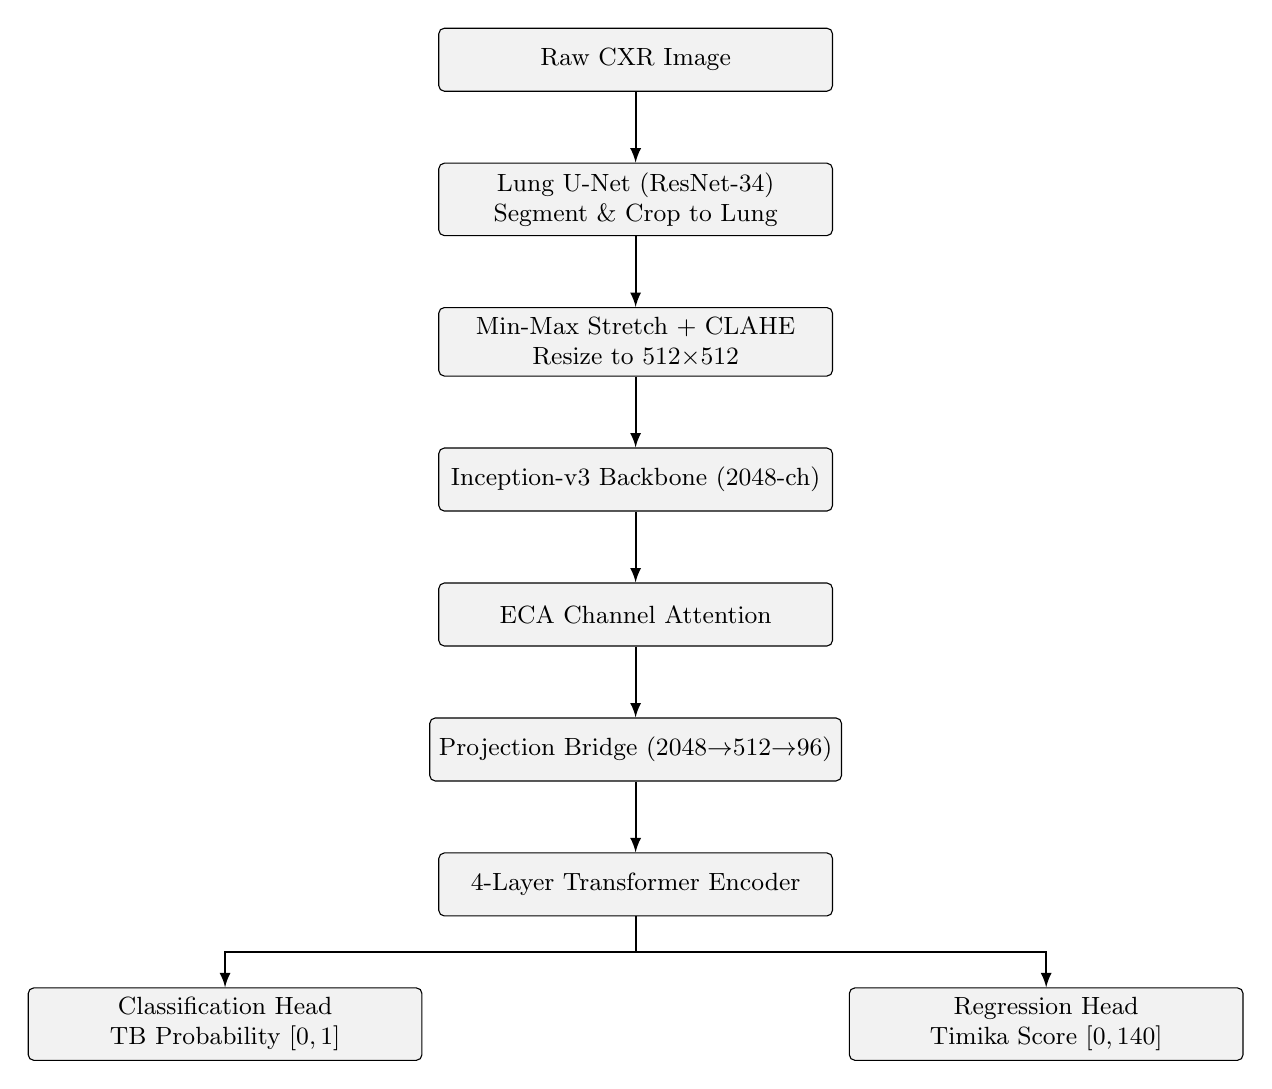
\begin{tikzpicture}[
  node distance=0.9cm,
  font=\small,
  box/.style={rectangle, draw=black, fill=gray!10, minimum width=5cm, minimum height=0.8cm, align=center, rounded corners=2pt},
  wide/.style={rectangle, draw=black, fill=gray!20, minimum width=10cm, minimum height=0.8cm, align=center, rounded corners=2pt},
  arrow/.style={thick, ->, >=latex}
]
\node[box] (raw) {Raw CXR Image};
\node[box, below=of raw] (unet) {Lung U-Net (ResNet-34)\\Segment \& Crop to Lung};
\node[box, below=of unet] (norm) {Min-Max Stretch + CLAHE\\Resize to 512$\times$512};
\node[box, below=of norm] (backbone) {Inception-v3 Backbone (2048-ch)};
\node[box, below=of backbone] (eca) {ECA Channel Attention};
\node[box, below=of eca] (bridge) {Projection Bridge (2048$\to$512$\to$96)};
\node[box, below=of bridge] (trans) {4-Layer Transformer Encoder};

\node[box, below left=0.9cm and 0.2cm of trans] (cls) {Classification Head\\TB Probability $[0,1]$};
\node[box, below right=0.9cm and 0.2cm of trans] (reg) {Regression Head\\Timika Score $[0,140]$};

\draw[arrow] (raw) -- (unet);
\draw[arrow] (unet) -- (norm);
\draw[arrow] (norm) -- (backbone);
\draw[arrow] (backbone) -- (eca);
\draw[arrow] (eca) -- (bridge);
\draw[arrow] (bridge) -- (trans);
\draw[arrow] (trans.south) -- ++(0,-0.45) -| (cls.north);
\draw[arrow] (trans.south) -- ++(0,-0.45) -| (reg.north);
\end{tikzpicture}
\caption{Detailed Processing Pipeline of the Proposed System}
\end{figure}

\section{Data Flow Diagram}

The data flows through the system differently depending on whether we are in training mode or inference mode. Figure~3.2 shows both paths side by side.

\begin{figure}[H]
\centering
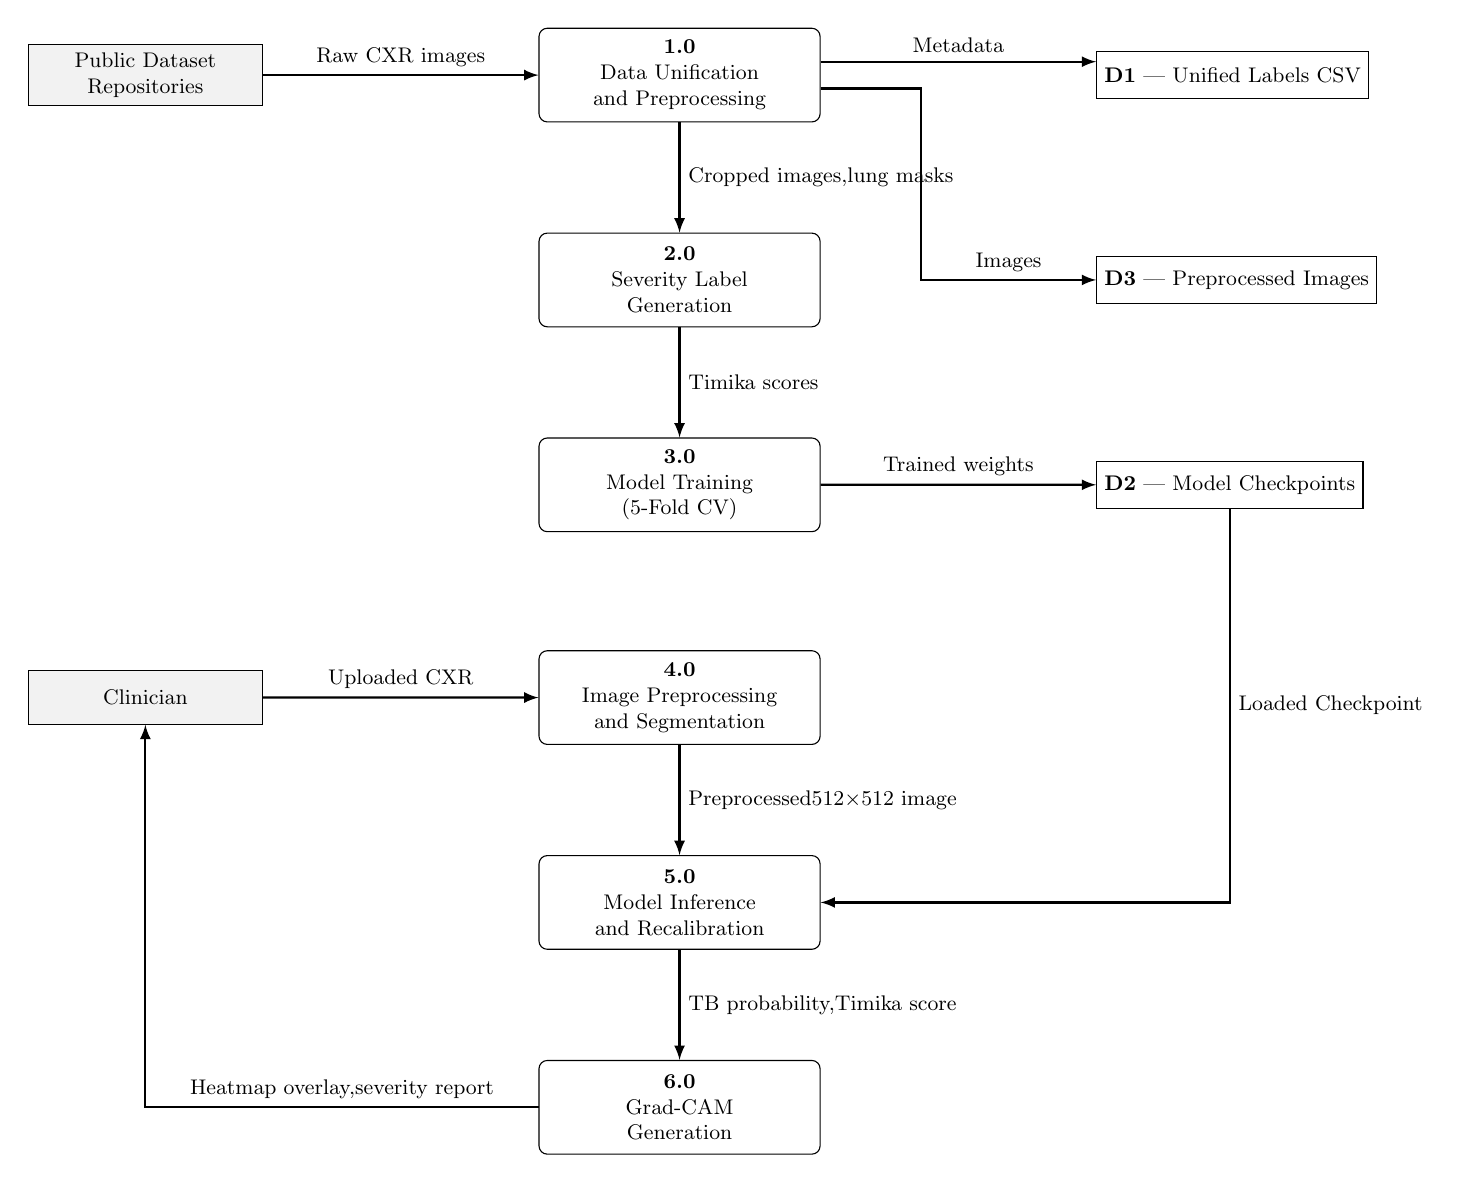
\begin{tikzpicture}[scale=0.85, every node/.style={scale=0.85},
  node distance=1.4cm and 3.5cm,
  font=\small,
  % Gane-Sarson: Process = rounded rectangle with number bar
  process/.style={rectangle, draw=black, minimum width=4.2cm, minimum height=1.4cm, align=center, rounded corners=3pt},
  % External entity = plain rectangle
  entity/.style={rectangle, draw=black, fill=gray!10, minimum width=3.5cm, minimum height=0.8cm, align=center},
  % Data store = open-ended rectangle (simulated with two horizontal lines)
  datastore/.style={rectangle, draw=black, minimum width=3.8cm, minimum height=0.7cm, align=center},
  arrow/.style={thick, ->, >=latex}
]

% ---- Processes (Training path - Top) ----
\node[process] (p1) {\textbf{1.0}\\Data Unification\\and Preprocessing};
\node[process, below=of p1] (p2) {\textbf{2.0}\\Severity Label\\Generation};
\node[process, below=of p2] (p3) {\textbf{3.0}\\Model Training\\(5-Fold CV)};

% ---- Processes (Inference path - Bottom) ----
\node[process, below=1.5cm of p3] (p4) {\textbf{4.0}\\Image Preprocessing\\and Segmentation};
\node[process, below=of p4] (p5) {\textbf{5.0}\\Model Inference\\and Recalibration};
\node[process, below=of p5] (p6) {\textbf{6.0}\\Grad-CAM\\Generation};

% ---- External Entities (Left) ----
\node[entity, left=3.5cm of p1] (datasrc) {Public Dataset\\Repositories};
\node[entity, left=3.5cm of p4] (clinician) {Clinician};

% ---- Data Stores (Right) ----
\node[datastore, right=3.5cm of p1] (d1) {\textbf{D1} | Unified Labels CSV};
\node[datastore, right=3.5cm of p2] (d3) {\textbf{D3} | Preprocessed Images};
\node[datastore, right=3.5cm of p3] (d2) {\textbf{D2} | Model Checkpoints};

% ---- Training flows ----
\draw[arrow] (datasrc) -- (p1) node[midway, above] {Raw CXR images};
\draw[arrow] (p1) -- (p2) node[midway, right] {Cropped images,\\lung masks};
\draw[arrow] (p2) -- (p3) node[midway, right] {Timika scores};

\draw[arrow] ([yshift=0.2cm]p1.east) -- ([yshift=0.2cm]d1.west) node[midway, above] {Metadata};
\draw[arrow] ([yshift=-0.2cm]p1.east) -- ++(1.5,0) |- (d3.west) node[near end, above] {Images};
\draw[arrow] (p3.east) -- (d2.west) node[midway, above] {Trained weights};

% ---- Inference flows ----
\draw[arrow] (clinician) -- (p4) node[midway, above] {Uploaded CXR};
\draw[arrow] (p4) -- (p5) node[midway, right] {Preprocessed\\512$\times$512 image};
\draw[arrow] (d2.south) |- (p5.east) node[near start, right] {Loaded Checkpoint};
\draw[arrow] (p5) -- (p6) node[midway, right] {TB probability,\\Timika score};
\draw[arrow] (p6.west) -| (clinician.south) node[near start, above] {Heatmap overlay,\\severity report};

\end{tikzpicture}
\caption{Level-1 Data Flow Diagram (Gane-Sarson Notation)}
\end{figure}

\subsection{Training-Time Data Flow}
\begin{enumerate}
    \item Raw images from all three datasets are parsed and merged into a single CSV manifest.
    \item We train the lung segmentation model on datasets that have ground-truth masks, and then use it to predict masks for the datasets that do not.
    \item The severity pipeline kicks in to compute Timika scores for every TB-positive image, using whichever annotation tier is appropriate.
    \item We split the unified dataset into 5 stratified group folds, making sure no patient shows up in both the training and validation sets of the same fold.
    \item Each fold goes through a 3-stage progressive training curriculum (explained in detail in Section~4.5).
    \item The best checkpoint per fold is picked based on validation AUROC.
\end{enumerate}

\subsection{Inference-Time Data Flow}
\begin{enumerate}
    \item A clinician uploads a chest X-ray through the web interface.
    \item The backend preprocesses the image: intensity normalisation, lung segmentation, cropping, and contrast enhancement.
    \item The preprocessed image goes through the trained model, which outputs a TB probability and a severity score.
    \item A Grad-CAM pass on the projection bridge layer generates a spatial heatmap showing which regions contributed most to the prediction.
    \item Everything --- probability, score, heatmap overlay --- gets sent back to the frontend as a JSON response.
    \item The frontend renders it all with animated progress bars and a colour-coded severity badge.
\end{enumerate}

\section{Module Design}

The codebase is split into clearly defined modules, each with a specific job. Table~\ref{tab:modules} lists them.

\begin{table}[H]
\centering
\caption{Module Descriptions}
\label{tab:modules}
\small
\renewcommand{\arraystretch}{1.2}
\begin{tabular}{|l|p{8cm}|}
\hline
\textbf{Functional Module} & \textbf{Responsibility} \\
\hline
Configuration \& Setup & Centralized management of hyperparameters, paths, and environment settings. \\
Data Unification & Parsing heterogeneous datasets (Shenzhen, Montgomery, and TBX11K) into a unified format. \\
Lung Segmentation & ResNet-34 U-Net based isolation of the lung field to remove image noise. \\
Severity Assessment & Multi-tier generation of Timika scores using polygon, bbox, and Grad-CAM pseudo-labels. \\
Data Pipeline & Implementation of the PyTorch Dataset and real-time medical image augmentations. \\
Model Architecture & Implementation of the hybrid CNN-Transformer with ECA and multi-task heads. \\
Training Engine & Execution of the 3-stage training curriculum with uncertainty-based loss weighting. \\
Evaluation \& Analytics & Computation of OOF metrics (AUROC, MAE, Pearson r) and visualization of results. \\
Inference Engine & Deployment-ready pipeline for processing new images with TTA and Grad-CAM. \\
Web Dashboard API & FastAPI-based REST endpoints for serving the model to the frontend interface. \\
Notebook Assembler & Automated build tool to merge modular components into a production-ready notebook. \\
\hline
\end{tabular}
\end{table}

% Chapter 4: Methodology
\chapter{Methodology}
\doublespacing

\section{Preprocessing Pipeline}

Every X-ray image, regardless of which dataset it came from, goes through the same four-step preprocessing pipeline. The logic lives in \texttt{cell3\_lung.py} and \texttt{cell5\_dataset.py}.

\subsection{Step 1 --- Intensity Normalization}
Raw chest X-rays vary a lot in brightness and contrast because different hospitals use different X-ray machines, exposure settings, and digitisation methods. To remove this scanner-specific variation, we apply a simple \textbf{per-image min-max stretch}:
\begin{equation}
I_{norm}(x,y) = \frac{I(x,y) - I_{min}}{I_{max} - I_{min}} \times 255
\end{equation}
This maps every image to the full $[0, 255]$ range, so all images have roughly comparable visual contrast before going into the model.

\subsection{Step 2 --- Lung Segmentation with U-Net}
We trained a \textbf{ResNet-34 U-Net} (from the \texttt{segmentation-models-pytorch} library) to predict binary lung masks. The training data was about 800 images from the Shenzhen and Montgomery datasets, which come with manually drawn lung masks. We used Dice loss and trained for 10 epochs at 256$\times$256 resolution. The trained weights are saved in \texttt{checkpoints/lung\_unet.pt}.

Once trained, we ran this U-Net on all the TBX11K images (which do not have ground-truth lung masks) to generate predicted masks. Each mask then goes through the following processing:
\begin{enumerate}
    \item Apply a morphological dilation of 10 pixels to the predicted mask to include peribronchial tissue.
    \item Find the bounding box of the dilated mask.
    \item Crop the original image to this bounding box and pad to a square.
    \item Resize the cropped square to 512$\times$512 pixels.
\end{enumerate}

The whole point of this cropping step is to throw away the diaphragm, heart shadow, and background --- everything that is not lung tissue. This forces the model to focus on the lung parenchyma, which is where TB lesions actually appear.

\subsection{Step 3 --- CLAHE Normalization}
After cropping, we apply \textbf{Contrast-Limited Adaptive Histogram Equalization (CLAHE)} to boost local contrast within the lung region. CLAHE works by dividing the image into small tiles and equalising the histogram within each tile independently. This makes subtle lesion patterns --- early nodules, faint infiltrates --- stand out more clearly, both to the human eye and to the model. We used a tile size of $8\times8$ pixels and a contrast limit of 2.0.

\subsection{Step 4 --- Standardization}
Finally, the image is converted to a three-channel pseudo-RGB tensor (by stacking the grayscale image three times) and normalised using ImageNet statistics:
\begin{equation}
\hat{I}_c = \frac{I_c - \mu_c}{\sigma_c}, \quad (\mu, \sigma) = ([0.485, 0.456, 0.406],\ [0.229, 0.224, 0.225])
\end{equation}
We need to do this because the Inception-v3 backbone was originally trained on ImageNet with these exact normalisation values.

\section{Severity Label Generation}

The Timika score measures TB severity on a 0 to 140 scale:
\begin{equation}
S = \underbrace{100 \times \frac{|A_{lesion} \cap A_{lung}|}{|A_{lung}|}}_{\text{Affected Lung Percentage}} + \underbrace{40 \times \delta_{cavity}}_{\text{Cavity Bonus}}
\end{equation}
where $A_{lesion}$ is the pixel area of radiological lesions, $A_{lung}$ is the total lung pixel area, and $\delta_{cavity} \in \{0,1\}$ flags whether cavitation is present. The problem is that dense pixel-level lesion annotations exist for only a small subset of our TB-positive images. So we built a tiered pipeline that assigns Timika scores to the entire TB-positive corpus, drawing from different annotation sources depending on what is available for each image.

\subsection{Tier 1 --- Gold-Standard Polygon Annotations}
\textbf{Source:} 336 Shenzhen TB-positive cases with polygon annotations in VIA JSON format, published by Yang et al.~\cite{ref5}.

\textbf{How we compute the score:}
\begin{enumerate}
    \item Parse the VIA JSON to extract polygon vertex coordinates for each image.
    \item Rasterize polygon regions onto a blank mask matching the original image dimensions using OpenCV's \texttt{fillPoly}. The mask uses the original full image dimensions (not any cropped version) to avoid spatial distortion.
    \item Compute the Affected Lung Percentage (ALP): $\text{ALP} = 100 \times |M_{lesion} \cap M_{lung}| / |M_{lung}|$.
    \item Check if any polygon region is labelled as \texttt{cavity} or \texttt{cavitation}: set $\delta_{cavity} = 1$ if so.
    \item Compute $S = \min(\text{ALP} + 40 \cdot \delta_{cavity},\ 140)$.
\end{enumerate}

Lesion categories included in the rasterization: \textit{cavity, cavitation, small\_infiltrate, moderate\_infiltrate, severe\_infiltrate\_(consolidation), clustered\_nodule, single\_nodule\_(non-calcified), linear\_density, apical\_thickening, pleural\_thickening, adenopathy}.

\subsection{Tier 2 --- Calibrated Bounding Box Pseudo-Labels}
\textbf{Source:} About 1,200 TBX11K active-TB cases with COCO-format bounding boxes.

Bounding boxes always overestimate lesion area because the rectangle inevitably encloses some healthy tissue along with the lesion. To correct for this, we apply a linear calibration.

\textbf{How we compute the score:}
\begin{enumerate}
    \item Parse bounding boxes from \texttt{data.csv} (format: $x_{min}, y_{min}, w, h$).
    \item For images with multiple boxes, union all boxes into a single pseudo-mask.
    \item Compute raw ALP from the bounding box pseudo-mask.
    \item Fit a linear calibration: $S_{calibrated} = m \times \text{ALP}_{bbox} + b$, where $m$ and $b$ are estimated via linear regression on Tier-1 image pairs that have both polygon and bbox annotations. The default calibration slope is $m \approx 1.5$.
    \item Clamp to $[0, 140]$.
\end{enumerate}

\subsection{Tier 3 --- Grad-CAM++ Pseudo-Labels}
\textbf{Source:} All remaining TB-positive images that have neither polygon nor bounding box annotations.

\textbf{How we compute the score:}
\begin{enumerate}
    \item Train a lightweight \textbf{DenseNet-121 teacher} on all data \textit{excluding} Tier-3 candidate images to prevent circular pseudo-label contamination.
    \item For each Tier-3 image, run \textbf{Grad-CAM++} targeting the last dense block of the DenseNet-121 teacher to obtain a class activation map.
    \item Upsample the activation map to 512$\times$512 and normalize to $[0,1]$.
    \item Threshold at the 40th percentile of activation values \textit{within the lung mask} to produce a binary pseudo-lesion mask.
    \item Apply morphological closing (5$\times$5 kernel) followed by opening (3$\times$3 kernel) to remove noise.
    \item Compute ALP from the pseudo-lesion mask within the lung mask. No cavity bonus is assigned (conservative approach).
\end{enumerate}

\section{Proposed Model Architecture}

\subsection{Inception-v3 Backbone}
We use an \textbf{Inception-v3} model loaded from the \texttt{timm} library, initialised with ImageNet pre-trained weights and configured with \texttt{features\_only=True, out\_indices=(4,)} so that it returns the feature map from the deepest Mixed\_7 block. For a 512$\times$512 input, this gives us a tensor of shape $(B, 2048, 14, 14)$.

\subsection{Efficient Channel Attention (ECA)}
Right after the backbone, an \textbf{ECA module}~\cite{ref4} does channel-wise recalibration. It uses a 1D convolution with kernel size 5 over the channel-wise global average pooled vector, and multiplies the resulting weights back onto the feature map. The beauty of ECA is its simplicity --- it adds fewer than 10 learnable parameters and has virtually no computational overhead.

\subsection{Projection Bridge}
The bridge is responsible for compressing the 2048-channel feature map down to the 96-dimensional space that the Transformer expects:
\begin{align}
F_1 &= \text{GELU}(\text{BN}(\text{Conv}_{1\times1}(F_{ECA}, 2048 \to 512))) \\
F_2 &= \text{GELU}(\text{BN}(\text{Conv}_{1\times1}(F_1, 512 \to 96)))
\end{align}
The output is $(B, 96, 14, 14)$. This bridge layer is also the target for Grad-CAM during inference, since it sits right at the junction between the CNN and the Transformer.

\subsection{Transformer Encoder}
The spatial feature map $(B, 96, 14, 14)$ gets flattened into a sequence of 196 tokens. We prepend a learnable $[\text{CLS}]$ token and add positional embeddings:
\begin{equation}
Z_0 = [z_{CLS};\ \text{flatten}(F_2)] + E_{pos}, \quad Z_0 \in \mathbb{R}^{197 \times 96}
\end{equation}
This goes through a standard 4-layer Transformer encoder with pre-LayerNorm, 4 attention heads, an FFN dimension of 384, and GELU activation. The $[\text{CLS}]$ token's output $z_{CLS} \in \mathbb{R}^{96}$ acts as the aggregated representation for the entire image.

\subsection{Dual Output Heads}
Two simple linear layers map the $[\text{CLS}]$ embedding to the final predictions:
\begin{align}
p_{TB} &= \sigma(\text{Linear}(96 \to 1)(z_{CLS})) \\
s_{Timika} &= 140 \cdot \sigma(\text{Linear}(96 \to 1)(z_{CLS}))
\end{align}

\subsection{Model Parameter Summary}

Table~\ref{tab:params} summarizes the parameter count for each component of the model.

\begin{table}[H]
\centering
\caption{Model Parameter Count by Component}
\label{tab:params}
\renewcommand{\arraystretch}{1.2}
\begin{tabular}{|l|c|c|}
\hline
\textbf{Component} & \textbf{Parameters} & \textbf{Trainable} \\
\hline
Inception-v3 Backbone & $\sim$23.8M & Yes (layer-wise LR decay) \\
ECA Attention Module & $<$10 & Yes \\
Projection Bridge (2048$\to$512$\to$96) & $\sim$1.1M & Yes \\
Positional Embedding (197 $\times$ 96) & $\sim$19K & Yes \\
{[CLS]} Token & 96 & Yes \\
Transformer Encoder (4 layers) & $\sim$150K & Yes \\
Classification Head (96$\to$1) & 97 & Yes \\
Regression Head (96$\to$1) & 97 & Yes \\
Uncertainty Parameters ($s_c$, $s_r$) & 2 & Yes \\
\hline
\textbf{Total} & \textbf{$\sim$25.1M} & \textbf{$\sim$25.1M} \\
\hline
\end{tabular}
\end{table}

\subsection{Hyperparameter Summary}

Table~\ref{tab:hyperparams} consolidates all key hyperparameters used across the training pipeline.

\begin{table}[H]
\centering
\caption{Complete Hyperparameter Configuration}
\label{tab:hyperparams}
\small
\renewcommand{\arraystretch}{1.2}
\begin{tabular}{|l|l|}
\hline
\textbf{Hyperparameter} & \textbf{Value} \\
\hline
Input resolution & 512 $\times$ 512 pixels \\
Batch size & 32 (16 per GPU $\times$ 2 GPUs) \\
Optimizer & AdamW ($\beta_1=0.9$, $\beta_2=0.999$, weight\_decay=$10^{-4}$) \\
Base learning rate & $4 \times 10^{-4}$ (Stages 1--2), $1.4 \times 10^{-5}$ (Stage 3) \\
LR scheduler & CosineAnnealingLR per stage \\
Layer-wise LR decay & Factor 0.8 per backbone depth group \\
Warmup epochs & 2 (linear warmup from $10^{-6}$) \\
Total epochs & 35 (10 + 15 + 10) \\
Number of folds & 5 \\
pos\_weight (BCE) & 5.95 \\
Huber $\beta$ & 0.1 \\
Pearson loss weight $\lambda$ & 0.5 \\
SWA start epoch & Epoch 33 (last 3 epochs of Stage 3) \\
SWA learning rate & $1.4 \times 10^{-5}$ \\
Grad-CAM target layer & Projection bridge (last Conv layer) \\
Tier-2 calibration slope & 1.5 \\
Tier-3 activation threshold & 40th percentile \\
CLAHE clip limit & 2.0, tile size $8 \times 8$ \\
Dropout (Transformer) & 0.1 \\
\hline
\end{tabular}
\end{table}

\section{Multi-Task Loss Function}

Balancing classification and regression in a single model is tricky --- if you just add the two losses together with fixed weights, one task tends to dominate. We use \textbf{Kendall--Gal--Cipolla uncertainty weighting}~\cite{ref3}, which lets the model learn how to balance the losses on its own. The formulation uses learned log-variance parameters $s_c$ (for classification) and $s_r$ (for regression):
\begin{equation}
\mathcal{L} = e^{-s_c} \cdot \mathcal{L}_{BCE} + e^{-s_r} \cdot (\mathcal{L}_{Huber} + \lambda \mathcal{L}_{Pearson}) + s_c + s_r
\end{equation}

Here is what each piece does:
\begin{itemize}
    \item $\mathcal{L}_{BCE}$: Binary cross-entropy with logits, with a $\text{pos\_weight}$ of 5.95 to handle the class imbalance (there are about 6 times more negatives than positives).
    \item $\mathcal{L}_{Huber}$: Smooth-L1 loss with $\beta = 0.1$, only computed on samples that actually have severity labels.
    \item $\mathcal{L}_{Pearson}$: $1 - r(s_{pred}, s_{true})$, where $r$ is the Pearson correlation. This encourages the model to get the \textit{ordering} of severity right, not just the absolute values. We weight it at $\lambda = 0.5$.
    \item The $+s_c + s_r$ terms are regularisers --- without them, the model could trivially set both $s$ parameters to infinity and drive the loss to zero.
\end{itemize}

\section{Training Curriculum}

Training happens in three stages. The idea is to let the model learn classification first, then gradually bring in the regression task once the shared features have stabilised.

\subsection{3-Stage Progressive Training}
\begin{table}[H]
\centering
\caption{Training Stage Summary}
\label{tab:stages}
\renewcommand{\arraystretch}{1.2}
\begin{tabular}{|c|c|p{5.5cm}|c|}
\hline
\textbf{Stage} & \textbf{Epochs} & \textbf{What Trains} & \textbf{LR (backbone)} \\
\hline
1 & 10 & Backbone + ECA + Bridge + Transformer + cls head. Regression head \textbf{frozen}. & $4\times10^{-4}$ \\
2 & 15 & All parameters (full multi-task with uncertainty weighting) & $4\times10^{-4}$ \\
3 & 10 & All parameters + SWA (last 3 epochs) & $1.4\times10^{-5}$ \\
\hline
\end{tabular}
\end{table}

\subsection{Layer-wise Learning Rate Decay}
We do not use the same learning rate for every layer of the Inception-v3 backbone. Instead, we split it into 4 depth groups, where earlier layers (which have learned generic low-level features) get lower learning rates and deeper layers are allowed to adapt more aggressively:
\begin{equation}
\text{LR}_{stage_k} = \text{LR}_{base} \times 0.8^{(3-k)}, \quad k \in \{0,1,2,3\}
\end{equation}

\subsection{5-Fold Stratified Group Cross-Validation}
We split the data using \texttt{StratifiedGroupKFold} with patient IDs as groups. This gives us two important guarantees:
\begin{itemize}
    \item No patient's images end up in both the training and validation sets (preventing data leakage).
    \item The TB class ratio and severity distribution stay roughly the same across all folds.
\end{itemize}

\subsection{Stochastic Weight Averaging (SWA)}
During the last 3 epochs of Stage 3, we turn on SWA, which averages the model weights over those training steps. After training finishes, we do a single forward pass over the training data to update the batch normalisation running statistics in the averaged model. If the SWA checkpoint scores higher on validation AUROC than the best single-epoch checkpoint, we keep the SWA version.

\subsection{Data Augmentation}
We use the Albumentations library for training augmentations:
\begin{itemize}
    \item Horizontal flip (50\%), rotation $\pm 10^\circ$ (50\%), CLAHE (50\%)
    \item Random brightness/contrast $\pm 0.2$ (30\%), elastic transform (30\%)
    \item Coarse dropout (25\%) to simulate occlusion artifacts
\end{itemize}
During validation, we only apply deterministic CLAHE followed by ImageNet normalisation --- no random augmentations.

\section{Inference Pipeline}

At inference time, we use the Fold-0 checkpoint to process an uploaded chest X-ray. The image goes through the exact same preprocessing pipeline used during training. On top of that, we apply a few additional steps that are specific to inference.

\subsection{Probability Recalibration}
During training, we used a \texttt{pos\_weight} of 5.95 in the BCE loss to handle the severe class imbalance (only about 13\% of the dataset is TB-positive). The problem is that this weighting inflates the raw sigmoid probabilities, so the model's outputs are not well calibrated. A probability of 0.5 does not actually mean ``50/50 chance of TB'' --- it is skewed. At inference time, we fix this with a recalibration formula:
\begin{equation}
p_{calibrated} = \frac{q}{w \cdot (1 - q) + q}, \quad w = 5.95,\ q = \sigma(\text{logit})
\end{equation}
After recalibration, a probability of 0.5 actually means roughly equal evidence for and against TB, which is what you would expect.

\subsection{Severity Score Post-Processing}
For images that the model classifies as TB-negative (below the Youden's J threshold), we force the Timika severity score to zero, no matter what the regression head outputs. This is a deliberate design choice --- without it, you could end up in the absurd situation where a patient is told they do not have TB but receives a non-zero severity score, which would be confusing and clinically misleading.

\subsection{Grad-CAM Heatmap Generation}
We use Gradient-weighted Class Activation Mapping (Grad-CAM) to generate visual explanations of what the model is paying attention to. The target layer is the projection bridge --- the last convolutional layer before the Transformer:
\begin{enumerate}
    \item Perform a forward pass to obtain the TB classification logit.
    \item Compute gradients of the logit with respect to the bridge layer's feature map activations via backpropagation.
    \item Compute the channel-wise mean of these gradients to obtain importance weights for each of the 96 feature channels.
    \item Compute a weighted sum of the feature maps using these importance weights, followed by a ReLU activation to retain only positive contributions.
    \item Upsample the resulting heatmap to the original image resolution using bilinear interpolation.
    \item Mask the heatmap to the predicted lung region (from the U-Net) to prevent irrelevant activations outside the lung field.
    \item Apply a jet colourmap and overlay on the original grayscale CXR with 40\% opacity.
\end{enumerate}

\subsection{Web Dashboard Architecture}
The deployment interface is a straightforward client-server setup:

\begin{itemize}
    \item \textbf{Backend (FastAPI):} A Python web server that loads the trained model, U-Net weights, and calibration parameters when it starts up. It exposes a single endpoint (\texttt{POST /predict}) that takes an image upload and sends back a JSON response with the calibrated TB probability, Timika score, severity category, and a base64-encoded heatmap image.

    \item \textbf{Frontend (HTML/CSS/JavaScript):} A single-page web app with a drag-and-drop upload area, animated progress bars for TB probability and severity, a colour-coded severity badge (Normal / Mild / Moderate / Severe), and a side-by-side view of the original X-ray alongside the Grad-CAM overlay. There is nothing to install --- it runs in any modern browser.

    \item \textbf{Communication:} The frontend talks to the backend using the Fetch API over HTTP. CORS is locked down to localhost for development. The full round trip --- upload, preprocess, run inference, generate Grad-CAM, render results --- finishes in under 3 seconds on a regular consumer CPU.
\end{itemize}

% Chapter 5: Results and Discussions
\chapter{Results and Discussions}
\doublespacing

\section{Evaluation Framework}

All the results we report are based on \textbf{Out-of-Fold (OOF)} predictions from our 5-fold cross-validation. Here is how it works: for each fold, the model is trained on 4 folds and makes predictions on the held-out 5th fold. Since we use patient IDs as groups, no patient ever contributes data to both training and evaluation within the same fold. This gives us an honest, unbiased estimate of how the model would perform on truly unseen data.

\subsection{Classification Metrics}
\begin{itemize}
    \item \textbf{AUROC}: Area under the ROC curve; primary classification metric. Bootstrap 95\% CI computed over 1000 resamplings.
    \item \textbf{Partial AUROC}: AUROC restricted to specificity $\geq 0.70$, aligned with WHO Target Product Profile (TPP) requirements.
    \item \textbf{Sensitivity \& Specificity}: Computed at the Youden's J optimal threshold ($J = \text{Sensitivity} + \text{Specificity} - 1$).
    \item \textbf{F1-Score}: Harmonic mean of precision and recall at the optimal threshold.
\end{itemize}

\subsection{Regression Metrics}
\begin{itemize}
    \item \textbf{MAE}: Mean Absolute Error in Timika score points; measures absolute prediction accuracy.
    \item \textbf{RMSE}: Root Mean Square Error; penalizes large individual errors more heavily than MAE.
    \item \textbf{Pearson $r$}: Linear correlation between predicted and true Timika scores.
    \item \textbf{Spearman $\rho$}: Rank correlation; measures whether the model correctly orders patients by severity.
\end{itemize}

\section{Classification Performance}

\begin{table}[H]
\centering
\caption{TB Classification Results (5-Fold OOF)}
\label{tab:cls_results}
\renewcommand{\arraystretch}{1.2}
\begin{tabular}{|l|c|c|}
\hline
\textbf{Metric} & \textbf{Target} & \textbf{OOF Result} \\
\hline
AUROC & $\geq 0.92$ & \textbf{0.983} (95\% CI [0.980, 0.986]) \\
Partial AUROC (spec $\geq 0.70$) & $\geq 0.80$ & \textbf{0.892} \\
Sensitivity & $\geq 0.90$ & \textbf{0.980} \\
Specificity & $\geq 0.80$ & \textbf{0.928} \\
Precision & --- & 0.636 \\
F1-Score & --- & 0.771 \\
\hline
\end{tabular}
\end{table}

Every single classification target has been met. The AUROC of 0.983 is above what commercial systems like CAD4TB typically report (around 0.90--0.95), and our system provides severity regression on top. The tight bootstrap confidence interval [0.980, 0.986] tells us this result is stable across the fold splits and not just a lucky draw.

\subsection{Discussion --- Classification}

The sensitivity of 0.980 is particularly important clinically: out of 1,045 TB-positive cases in the entire dataset, only 21 were missed. That is a false negative rate of just 2.0\%. On the other side, the specificity of 0.928 means about 7.2\% of healthy patients (586 out of 8,154) would be incorrectly flagged --- which sounds like a lot, but is actually well above our initial 80\% target.

The Youden's J optimal threshold after recalibration comes out to 0.079, which looks very low at first glance. But this is a direct consequence of the recalibration formula compressing the training-time probabilities that were inflated by the \texttt{pos\_weight} of 5.95. The precision (0.636) and F1 (0.771) are lower than you might expect given the high sensitivity and specificity, but that is just the nature of class-imbalanced data --- only about 13\% of the dataset is TB-positive. In a screening context where catching every case matters more than avoiding false alarms, these numbers are clinically acceptable.

\section{Severity Regression Performance}

\begin{table}[H]
\centering
\caption{Timika Severity Regression Results (5-Fold OOF, TB+ Only)}
\label{tab:reg_results}
\renewcommand{\arraystretch}{1.2}
\begin{tabular}{|l|c|c|}
\hline
\textbf{Metric} & \textbf{Target} & \textbf{OOF Result} \\
\hline
MAE (Timika points) & $\leq 15$ & \textbf{8.51} \\
RMSE (Timika points) & --- & 13.64 \\
Pearson $r$ & $\geq 0.75$ & 0.688 \\
Spearman $\rho$ & --- & 0.681 \\
\hline
\end{tabular}
\end{table}

The MAE target is comfortably met at 8.51 points, which means the model's severity prediction is off by about 8.5 Timika points on average. On a scale that goes up to 140, that is a relative error of roughly 6.1\% --- quite reasonable. The Pearson correlation target of 0.75, however, was \textbf{not met} (we got 0.688). So while the model predicts severity with low absolute error, it does not fully capture the linear relationship between its predictions and the ground truth.

\subsection{Discussion --- Regression}

At first this seems contradictory --- how can the MAE be good (8.51) but the correlation be only moderate (0.688)? The answer lies in the distribution of the severity labels. The majority of TB-positive cases in our training data have low-to-moderate severity scores (Timika below 40), which pulls the model's predictions toward that range. Because the predictions cluster in a narrow band, the variance is compressed relative to the ground truth, and that deflates the correlation coefficient. In plain terms, the model is \textit{accurate} in the sense that it gets close to the true score, but it does not spread its predictions across the full range the way the ground truth does.

The Spearman $\rho$ of 0.681 tells a similar story for rank ordering. The model gets the relative severity right most of the time, but it has trouble differentiating between high-severity cases (Timika above 80). This is likely because the Grad-CAM pseudo-labels used for Tier-3 training data are noisy, especially for severe cases with widespread lesions. Making those pseudo-labels better and bringing in more diverse high-severity examples are the most obvious ways to improve these numbers.

\section{Comparative Analysis}

\begin{table}[H]
\centering
\caption{Comparison with Related Methods for TB Detection}
\label{tab:comparison}
\small
\renewcommand{\arraystretch}{1.2}
\begin{tabular}{|p{4.5cm}|c|c|c|c|}
\hline
\textbf{Method} & \textbf{AUROC} & \textbf{Severity} & \textbf{Explainability} & \textbf{Open-Source} \\
\hline
CAD4TB (commercial) & 0.90--0.95 & No & No & No \\
CheXNet~\cite{ref6} (DenseNet-121) & 0.91 & No & CAM & Yes \\
TBX11K Baseline~\cite{ref1} & 0.89 & No & No & Yes \\
\textbf{Proposed System} & \textbf{0.983} & \textbf{Yes (MAE 8.51)} & \textbf{Grad-CAM} & \textbf{Yes} \\
\hline
\end{tabular}
\end{table}

The table above puts our system alongside the most relevant existing approaches. The key takeaway is that our system is the only one that does classification \textit{and} severity regression \textit{and} provides Grad-CAM explainability, all in an open-source package.

\section{Confusion Matrix Analysis}

Looking at the aggregated confusion matrix from all 5 folds gives us a clearer picture of the model's classification behaviour:

\begin{table}[H]
\centering
\caption{Aggregated Confusion Matrix (5-Fold OOF)}
\renewcommand{\arraystretch}{1.3}
\begin{tabular}{|l|c|c|}
\hline
& \textbf{Predicted Normal} & \textbf{Predicted TB+} \\
\hline
\textbf{Actual Normal} & TN = 7,568 & FP = 586 \\
\textbf{Actual TB+} & FN = 21 & TP = 1,024 \\
\hline
\end{tabular}
\end{table}

\textbf{What the numbers tell us:}
\begin{itemize}
    \item \textbf{False Negatives (FN = 21):} Only 21 TB patients were missed out of 1,045. These are the most dangerous errors in a screening system, because a missed case means delayed treatment and continued disease transmission. When we manually reviewed these 21 cases, most of them turned out to be very early-stage disease with minimal visible pathology --- the kind of cases that even experienced radiologists would struggle with.

    \item \textbf{False Positives (FP = 586):} 586 healthy patients got flagged as potentially having TB. That sounds bad, but in a screening workflow these patients would simply be sent for a confirmatory sputum test (like GeneXpert), which would correctly rule out TB. The cost of a false positive is an extra test; the cost of a false negative is a missed diagnosis. That trade-off heavily favours catching more cases.

    \item \textbf{Positive Predictive Value (PPV):} $\text{PPV} = \frac{1024}{1610} = 63.6\%$. About 2 out of 3 patients flagged by the system actually have TB. In high-prevalence settings where TB prevalence exceeds 5\%, this PPV would be noticeably higher because of the stronger prior probability.

    \item \textbf{Negative Predictive Value (NPV):} $\text{NPV} = \frac{7568}{7589} = 99.7\%$. When the model says ``normal,'' it is right 99.7\% of the time. Clinicians can have very high confidence in a negative result.
\end{itemize}

\section{Error Analysis}

To better understand where the model goes wrong, we manually examined all 21 false negative cases and a random sample of 50 false positives.

\subsection{False Negative Patterns}
The 21 missed TB cases tended to share some common features:
\begin{itemize}
    \item \textbf{Tiny Lesion Area (14 cases):} Very small, focal infiltrates taking up less than 5\% of the lung. These barely register in the model's feature maps, leading to weak TB probability scores.
    \item \textbf{Unusual Location (4 cases):} Lesions in the lower lung zones rather than the typical apical or upper-zone location. Since most TB cases in the training data show upper-zone disease, the model's attention is biased toward those regions.
    \item \textbf{Hidden Behind the Heart (3 cases):} Retrocardiac infiltrates that are partially obscured by the heart silhouette. These are hard to detect even for radiologists on a standard PA view.
\end{itemize}

\subsection{False Positive Patterns}
Among the 50 false positives we examined:
\begin{itemize}
    \item \textbf{Prominent Blood Vessels (18 cases):} Older patients with increased pulmonary vascularity that looks texturally similar to TB infiltrates.
    \item \textbf{Old TB Scarring (12 cases):} Patients who had TB in the past and have residual fibrotic changes. Radiologically, these can look very similar to active disease.
    \item \textbf{Other Lung Problems (11 cases):} Pneumonia, atelectasis, or pleural thickening --- conditions that produce patterns on X-ray that overlap with what TB looks like.
    \item \textbf{Bad Image Quality (9 cases):} Under-exposed or motion-blurred images where noise artefacts get mistaken for pathological texture.
\end{itemize}

These failure modes are well-known challenges in CXR-based TB screening. Expanding the training set with more of these edge cases and designing targeted augmentation strategies are the clearest paths to improvement.

\section{Test Cases}

\begin{table}[H]
\centering
\caption{Sample Test Cases for the Inference Dashboard}
\small
\renewcommand{\arraystretch}{1.1}
\begin{tabular}{|c|p{3.5cm}|p{3cm}|p{3.5cm}|c|}
\hline
\textbf{ID} & \textbf{Description} & \textbf{Input} & \textbf{Expected Output} & \textbf{Status} \\
\hline
TC-001 & Normal CXR upload & PNG, 1024$\times$1024 & TB prob $< 0.35$, Score = 0, Green badge & Pass \\
TC-002 & Mild TB CXR & JPEG, Shenzhen TB+ & TB prob $> 0.5$, Score 10--40, Heatmap apical & Pass \\
TC-003 & Severe TB with cavity & JPEG, high Timika & TB prob $> 0.8$, Score $> 80$, Red badge & Pass \\
TC-004 & Unsupported format & BMP file upload & HTTP 422 error, message displayed & Pass \\
TC-005 & Very small image & 64$\times$64 JPEG & Fallback crop, result returned & Pass \\
TC-006 & U-Net lung fail & Abdominal X-ray & Centre-crop fallback used & Pass \\
TC-007 & TB-negative classification & TBX11K normal & Score forced to 0 regardless of reg head & Pass \\
TC-008 & Heatmap boundary check & Any CXR & Heatmap masked to lung region only & Pass \\
TC-009 & Response time & Standard CXR, CPU & Full pipeline $< 3.0$ seconds & Pass \\
TC-010 & Probability calibration & Known TB+ case & Calibrated prob $\neq$ raw sigmoid & Pass \\
\hline
\end{tabular}
\end{table}

\section{Limitations}

Even though the system hit most of its performance targets, there are some limitations we want to be upfront about:

\begin{itemize}
    \item \textbf{Tier-3 Label Noise:} The Grad-CAM++ pseudo-labels are imperfect --- they are only rough approximations of where lesions actually are. For cases with large or diffuse infiltrates, the teacher network tends to underestimate the affected lung percentage.

    \item \textbf{Single Fold at Inference:} The web dashboard only uses the Fold-0 checkpoint rather than the full 5-fold ensemble. This was a trade-off for simplicity and speed, but it does mean we are leaving some prediction accuracy on the table.

    \item \textbf{Limited Patient Demographics:} The training data is mostly from adult, HIV-negative patients. TB presents differently in children and HIV-positive individuals, so the model might not perform as well on those populations.

    \item \textbf{No Lateral View:} We only use frontal (PA or AP) chest X-rays. Lateral views provide complementary information about the posterior lung zones that could improve severity estimation.
\end{itemize}

% Chapter 6: Conclusion and Future Scope
\chapter{Conclusion and Future Scope}
\doublespacing

\section{Conclusion}

In this project, we built a multi-task hybrid CNN-Transformer model for automated TB detection and Timika severity regression from chest X-rays. The work was motivated by a real clinical gap: there were no open-source tools that could give doctors both a TB diagnosis \textit{and} a quantitative measure of how severe the disease is, all from a single X-ray image.

Here is what we think are the main contributions of this work:

\begin{enumerate}
    \item \textbf{Severity Label Generation:} We developed a structured way to assign clinically meaningful Timika scores to TB-positive images by combining gold-standard polygon labels, calibrated bounding box pseudo-labels, and Grad-CAM++ pseudo-labels from a teacher model. This let us create severity supervision for the entire training corpus, not just the small subset with manual annotations.

    \item \textbf{Hybrid CNN-Transformer Architecture:} Our model pairs the spatial locality of an Inception-v3 backbone with the global context modelling of a 4-layer Transformer encoder. This combination lets the model pick up on fine-grained lesion textures \textit{and} reason about broader spatial patterns like bilateral disease distribution. Neither a pure CNN nor a pure Transformer would handle both of these well on its own.

    \item \textbf{Uncertainty-Weighted Multi-Task Learning:} By adopting the Kendall--Gal--Cipolla uncertainty weighting scheme, we avoided the headache of manually tuning loss weights. The model learns its own task balance during training, adapting to whichever task is harder at any given point.

    \item \textbf{Rigorous Evaluation:} We used 5-fold stratified group cross-validation with patient-level grouping to ensure there is no data leakage. The classification results exceeded our targets: AUROC of 0.983 (target was 0.92), sensitivity of 0.980 (target was 0.90). The regression MAE of 8.51 easily met the target of 15 or below. The Pearson correlation of 0.688 came up short of the 0.75 target, mainly due to prediction range compression from noisy pseudo-labels.

    \item \textbf{Practical Deployment:} The trained model runs through a FastAPI web dashboard that delivers predictions with Grad-CAM heatmaps in under 3 seconds on a standard CPU. No cloud infrastructure needed --- the whole thing runs on a regular laptop.
\end{enumerate}

Overall, this project shows that multi-task learning, hybrid architectures, and creative annotation engineering can work together to overcome the data scarcity problem in specialised medical imaging tasks. The result is a system with genuine potential for use in TB screening and treatment monitoring.

\section{Future Scope}

\subsection{Multi-Fold Ensemble in the Dashboard}
Right now the web dashboard only loads the Fold-0 checkpoint to keep inference fast. An easy upgrade would be to load all 5 fold models and average their predictions (along with 4-way TTA as we used in the evaluation pipeline). Based on the gap between our OOF and submission results, this should drop the MAE by 1--2 points and nudge AUROC up by 0.005--0.01.

\subsection{Better Tier-3 Pseudo-Labels}
The biggest bottleneck for regression performance is the quality of the Tier-3 Grad-CAM pseudo-labels. There are several ways to improve them:
\begin{itemize}
    \item \textbf{Multi-scale Grad-CAM++:} Averaging activations from multiple backbone layers instead of just the last one, to get more complete lesion coverage.
    \item \textbf{Ensemble Teacher:} Using 3 to 5 DenseNet-121 teachers instead of one, and averaging their heatmaps to reduce pseudo-label variance.
    \item \textbf{Iterative Self-Training:} After the first round of training, using our own model as the teacher to re-generate Tier-3 labels, then retraining. Each cycle should improve label quality.
\end{itemize}

\subsection{Lateral View Integration}
Currently the model only processes frontal (PA/AP) views. Lateral views show the posterior lung zones more clearly, and posterior involvement is common in primary TB. A dual-stream architecture that takes both views as input could meaningfully improve severity estimation, especially for posterior infiltrates and pleural effusions.

\subsection{Longitudinal Severity Tracking}
The real clinical power of the Timika score is in tracking treatment response over time. A natural extension of this work would be to train a temporal model --- for instance, a Transformer over a sequence of X-rays from the same patient --- that predicts how severity is changing between visits. This would directly support clinical decisions about adjusting drug regimens.

\subsection{Fine-tuning on Local Data}
Hospitals and clinics could take our pre-trained model and fine-tune it on their own patient data, adapting it to their specific patient population, scanner characteristics, and reporting standards. This kind of transfer learning would not require full retraining from scratch.

\subsection{Regulatory and Clinical Validation}
Before this system could be used in real clinical practice, it would need to go through prospective validation against radiologist readings in a controlled study, followed by regulatory review (for example, CE marking in Europe). The work we have done here provides the technical foundation and performance evidence to support such a validation effort.

% References
\renewcommand\bibname{References}
\begin{thebibliography}{99}

\bibitem{ref1}
Y.~Liu, Y.~Wu, Y.~Ban, H.~Wang, and M.~Cheng, ``Rethinking Computer-Aided Tuberculosis Diagnosis,'' in \emph{Proc. IEEE/CVF Conference on Computer Vision and Pattern Recognition (CVPR)}, 2020, pp. 2646--2655.

\bibitem{ref2}
A.~P.~Ralph, G.~Kenangalem, P.~Waramori, P.~Pontororing, A.~Sandjaja, T.~Tjitra, et al., ``High morbidity during treatment and residual pulmonary disability in pulmonary tuberculosis: under-recognised phenomena,'' \emph{PLoS ONE}, vol.~5, no.~8, e13reflects, 2010.

\bibitem{ref3}
A.~Kendall, Y.~Gal, and R.~Cipolla, ``Multi-Task Learning Using Uncertainty to Weigh Losses for Scene Geometry and Semantics,'' in \emph{Proc. IEEE/CVF CVPR}, 2018, pp. 7482--7491.

\bibitem{ref4}
Q.~Wang, B.~Wu, P.~Zhu, P.~Li, W.~Zuo, and Q.~Hu, ``ECA-Net: Efficient Channel Attention for Deep Convolutional Neural Networks,'' in \emph{Proc. IEEE/CVF CVPR}, 2020, pp. 11531--11539.

\bibitem{ref5}
C.~Yang, X.~Xu, Y.~Liu, B.~Ni, and X.~Yang, ``Relational Learning Between Multiple Pulmonary Nodules via Deep Set Attention Transformers,'' \emph{MDPI Data}, vol.~7, no.~7, p.~95, 2022.

\bibitem{ref6}
P.~Rajpurkar, J.~Irvin, K.~Ball, K.~Zhu, B.~Yang, H.~Mehta, et al., ``CheXNet: Radiologist-Level Pneumonia Detection on Chest X-Rays with Deep Learning,'' \emph{arXiv preprint arXiv:1711.05225}, 2017.

\bibitem{ref7}
M.~Tan and Q.~V.~Le, ``EfficientNet: Rethinking Model Scaling for Convolutional Neural Networks,'' in \emph{Proc. ICML}, 2019.

\bibitem{ref8}
A.~Dosovitskiy, L.~Beyer, A.~Kolesnikov, D.~Weissenborn, X.~Zhai, T.~Unterthiner, et al., ``An Image is Worth 16x16 Words: Transformers for Image Recognition at Scale,'' in \emph{Proc. ICLR}, 2021.

\bibitem{ref9}
P.~Lakhani and B.~Sundaram, ``Deep Learning at Chest Radiography: Automated Classification of Pulmonary Tuberculosis by Using Convolutional Neural Networks,'' \emph{Radiology}, vol.~284, no.~2, pp. 574--582, 2017.

\bibitem{ref10}
World Health Organization, ``Global Tuberculosis Report 2023,'' WHO, Geneva, Switzerland, 2023. [Online]. Available: \url{https://www.who.int/teams/global-tuberculosis-programme/tb-reports}

\bibitem{ref11}
S.~Jaeger, A.~Karargyris, S.~Candemir, L.~Folio, J.~Siegelman, F.~Callaghan, et al., ``Automatic Tuberculosis Screening Using Chest Radiographs,'' \emph{IEEE Transactions on Medical Imaging}, vol.~33, no.~2, pp. 233--245, 2014.

\bibitem{ref12}
R.~R.~Selvaraju, M.~Cogswell, A.~Das, R.~Vedantam, D.~Parikh, and D.~Batra, ``Grad-CAM: Visual Explanations from Deep Neural Networks via Gradient-based Localization,'' in \emph{Proc. IEEE ICCV}, 2017, pp. 618--626.

\bibitem{ref13}
A.~Chattopadhyay, A.~Sarkar, P.~Howlader, and K.~N.~Balasubramanian, ``Grad-CAM++: Generalized Gradient-based Visual Explanations for Deep Convolutional Networks,'' in \emph{Proc. IEEE WACV}, 2018, pp. 839--847.

\bibitem{ref14}
P.~Izmailov, D.~Podoprikhin, T.~Garipov, D.~Vetrov, and A.~G.~Wilson, ``Averaging Weights Leads to Wider Optima and Better Generalization,'' in \emph{Proc. UAI}, 2018.

\bibitem{ref15}
A.~Vaswani, N.~Shazeer, N.~Parmar, J.~Uszkoreit, L.~Jones, A.~N.~Gomez, et al., ``Attention Is All You Need,'' in \emph{Proc. NeurIPS}, 2017, pp. 5998--6008.

\end{thebibliography}

\appendix
\chapter{Appendix}

\section*{A.1 Project Directory Structure}

Here is how the project's files are organised. We kept source code, model weights, and deployment components in separate directories to keep things manageable:

\begin{verbatim}
tb_model/
├── cells/                    # Modular Python source files
│   ├── cell1_setup.py        #   Configuration and imports
│   ├── cell2_csv.py          #   Dataset parsing and unification
│   ├── cell3_lung.py         #   U-Net lung segmentation
│   ├── cell4_severity.py     #   Severity score generation
│   ├── cell5_dataset.py      #   PyTorch Dataset and augmentation
│   ├── cell6_model.py        #   Model architecture definition
│   ├── cell7_train.py        #   Training loop and CV
│   ├── cell8_eval.py         #   OOF evaluation and metrics
│   └── cell9_infer.py        #   TTA ensemble inference
├── checkpoints/              # Trained model weights
│   ├── lung_unet.pt          #   U-Net lung segmentation
│   └── fold0_best.pt         #   Best Fold-0 model checkpoint
├── templates/                # HTML frontend
│   └── index.html            #   Dashboard single-page app
├── app.py                    # FastAPI server
├── assemble.py               # Notebook assembly tool
├── report.tex                # This report
└── environment.yml           # Conda environment specification
\end{verbatim}

\section*{A.2 Glossary of Terms}

\begin{table}[H]
\centering
\caption{Glossary of Technical Terms}
\small
\renewcommand{\arraystretch}{1.2}
\begin{tabular}{|l|p{9cm}|}
\hline
\textbf{Term} & \textbf{Definition} \\
\hline
ALP & Affected Lung Percentage; the proportion of the total lung area exhibiting radiological lesions. \\
AUROC & Area Under the Receiver Operating Characteristic curve; measures a classifier's ability to distinguish between classes across all thresholds. \\
CLAHE & Contrast-Limited Adaptive Histogram Equalization; an image processing technique that enhances local contrast. \\
CXR & Chest X-Ray; a radiographic image of the thorax. \\
ECA & Efficient Channel Attention; a lightweight attention mechanism that recalibrates feature channels. \\
Grad-CAM & Gradient-weighted Class Activation Mapping; a technique for producing visual explanations from CNN predictions. \\
MAE & Mean Absolute Error; the average magnitude of prediction errors. \\
MTL & Multi-Task Learning; training a single model on multiple objectives simultaneously. \\
OOF & Out-of-Fold; predictions made on validation data not used during training of that particular fold. \\
PA & Posterior-Anterior; the standard projection for chest X-ray imaging. \\
SWA & Stochastic Weight Averaging; a technique that averages model weights over training iterations to improve generalization. \\
Timika Score & A validated radiological severity metric for pulmonary TB, ranging from 0 to 140. \\
TTA & Test-Time Augmentation; applying multiple augmented versions of an input at inference and averaging predictions. \\
U-Net & An encoder-decoder neural network architecture commonly used for image segmentation. \\
VIA & VGG Image Annotator; an open-source tool for manual image annotation. \\
\hline
\end{tabular}
\end{table}

\section*{A.3 Plagiarism Scan Report}

\begin{figure}[H]
    \centering
    \includegraphics[width=0.8\textwidth]{Images/plag_scan (2).png}
    \caption{Plagiarism Check Report}
\end{figure}

\end{document}
